\documentclass{beamer}
\usepackage[utf8]{inputenc}
\usepackage[portuguese]{babel}
\usepackage{amsthm}
\usepackage{amssymb, bm}
\usepackage{ragged2e}
\usepackage{graphicx}
\usepackage{pythonhighlight}
\usepackage{float}


%%% Tema Customizado para o Beamer
\usefonttheme{serif}

\setbeamertemplate{footline}[frame number]{}
\setbeamertemplate{navigation symbols}{}
\setbeamertemplate{caption}[numbered]

\usecolortheme{lily}
\setbeamercolor{block title}{bg=blue!20,fg=black}
\setbeamercolor{block body}{bg = blue!10, fg = black}
\setbeamertemplate{itemize item}[square]
\setbeamercolor{itemize item}{fg = blue}
\setbeamercolor{enumerate item}{fg = blue}

\usetheme{default}
\beamertemplatenavigationsymbolsempty
\setbeamercolor{titlelike}{fg=blue}
%%%

\graphicspath{{./imagens/}}

\theoremstyle{definition}
\newtheorem{teorema}{Teorema}

\title{Classificação: \textit{Concrete Crack Images for Classification}}
\author{Carolina Dias}
\date{Junho de 2022}

\begin{document}

\maketitle

\begin{frame}{Conteúdo}
\begin{enumerate}
    \item Decomposição Espectral;
    \item Decomposição em Valores Singulares (SVD);
    \item Redução de Dimensionalidade;
    \item Conjunto de Dados: \textit{Concrete Crack};
    \item Experimentos e Resultados.
\end{enumerate}
\end{frame}


\begin{frame}{Decomposição Espectral}

\begin{teorema}
    Se uma matriz $A$ $n \times n$ possuir $n$ autovetores linearmente independentes, então $A$ será diagonalizável. A decomposição $$A = S\Lambda S^{-1}$$ é chamada de \textbf{decomposição espectral} (ou de autovalor) da matriz $A$, sendo $\Lambda$ uma matriz diagonal com os autovalores de $A$ em sua diagonal principal.
\end{teorema}
\end{frame}

\begin{frame}{Decomposição em Valores Singulares (SVD)}
    \textbf{SVD Reduzida}
    
    Queremos encontrar uma decomposição da forma

$$X = \hat{U}\hat{S}V^T$$

tal que

\begin{itemize}
    \item $\hat{U}$ é uma matriz $m \times n$, com colunas ortonormais, chamadas \textbf{vetores singulares esquerdos} de $X$;
    \item $\hat{S}$ é uma matriz $n \times n$ diagonal, onde seus elementos da diagonal principal são os \textbf{valores singulares} de $X$;
    \item $V$ é uma matriz $n \times n$ ortogonal, cujas colunas são os \textbf{vetores singulares direitos} de $X$ e representam os autovetores de $X^TX$.
\end{itemize}
\end{frame}

\begin{frame}{Decomposição em Valores Singulares (SVD)}
    Também vale que

\begin{equation*}
\hat{S} = 
\begin{bmatrix}
    \sigma_1 & \dots & 0 \\
    \vdots & \ddots & \vdots \\
    0 & \dots & \sigma_n
\end{bmatrix}
=
\begin{bmatrix}
    \sqrt{\lambda_1} & \dots & 0 \\
    \vdots & \ddots & \vdots \\
    0 & \dots & \sqrt{\lambda_n}
\end{bmatrix}
\end{equation*}

com $\sigma_1 \geq \sigma_2 \geq \dots \geq \sigma_n \geq 0$.
\end{frame}

\begin{frame}{Redução de Dimensionalidade}
    \begin{itemize}
        \item Calculamos a variabilidade acumulada $$E(r) = \frac{\lambda_1 + \lambda_2 + \dots + \lambda_r}{\lambda_1 + \lambda_2 + \dots + \lambda_n};$$
        \pause
        \item Encontramos um valor de $r$ com alta variabilidade acumulada;
        \pause
        \item Pegamos os $r$ primeiros autovetores (colunas) de $Q$ (respectivamente de $V$) para obter $\hat{Q}$ (e $\hat{V}$);
        \pause
        \item Multiplicamos matricialmente os dados originais por $\hat{Q}$ (e $\hat{V}$ obtendo, assim, as componentes principais;
        \pause
        \item Utilizamos apenas essas componentes principais para realizar a classificação, ao invés dos dados completos.
    \end{itemize}
\end{frame}

\begin{frame}{Conjunto de Dados: \textit{Concrete Crack}}

\begin{itemize}
    \item Classificação da existência de rachaduras em concreto;
    \item 40.000 imagens de concreto:
    \begin{itemize}
        \item 20.000 com rachaduras (\textit{positive}) e
        \item 20.000 sem rachaduras (\textit{negative}).
    \end{itemize}
    \item Imagens com $227 \times 227$ pixels, em 3 canais (RGB);
    \item Foram convertidas para imagens com $32 \times 32$ pixels com 1 canal (\textit{greyscale}).
\end{itemize}
\end{frame}

\begin{frame}{Experimentos e Resultados}
    \begin{enumerate}
        \item Cada imagem foi transformada em um vetor de $23 \times 32 = 1024$ características;
        \pause
        \item Todas foram armazenadas em uma tabela para facilitar sua manipulação;
        \pause
        \item Tabela separada em \textit{X\_train, y\_train, X\_test, y\_test};
        \pause
        \item Matrizes \textit{X\_train} e \textit{X\_test} foram centralizadas;
        \pause
        \item Calculada a covariância dos dados de teste.
        \item Autovalores e autovetores ordenados decrescentemente;
        \pause
        \item Calculada a decomposição espectral da matriz de covariância e a SVD de \textit{X\_train};
        \pause
        \item Gráficos gerados, $r$ escolhido e algoritmo KNN aplicado.
    \end{enumerate}
\end{frame}

\begin{frame}{Experimentos e Resultados}
\begin{figure}[H]
  \centering
    \caption{Gráfico da variabilidade acumulada por número de autovalores na Decomposição Espectral.}
    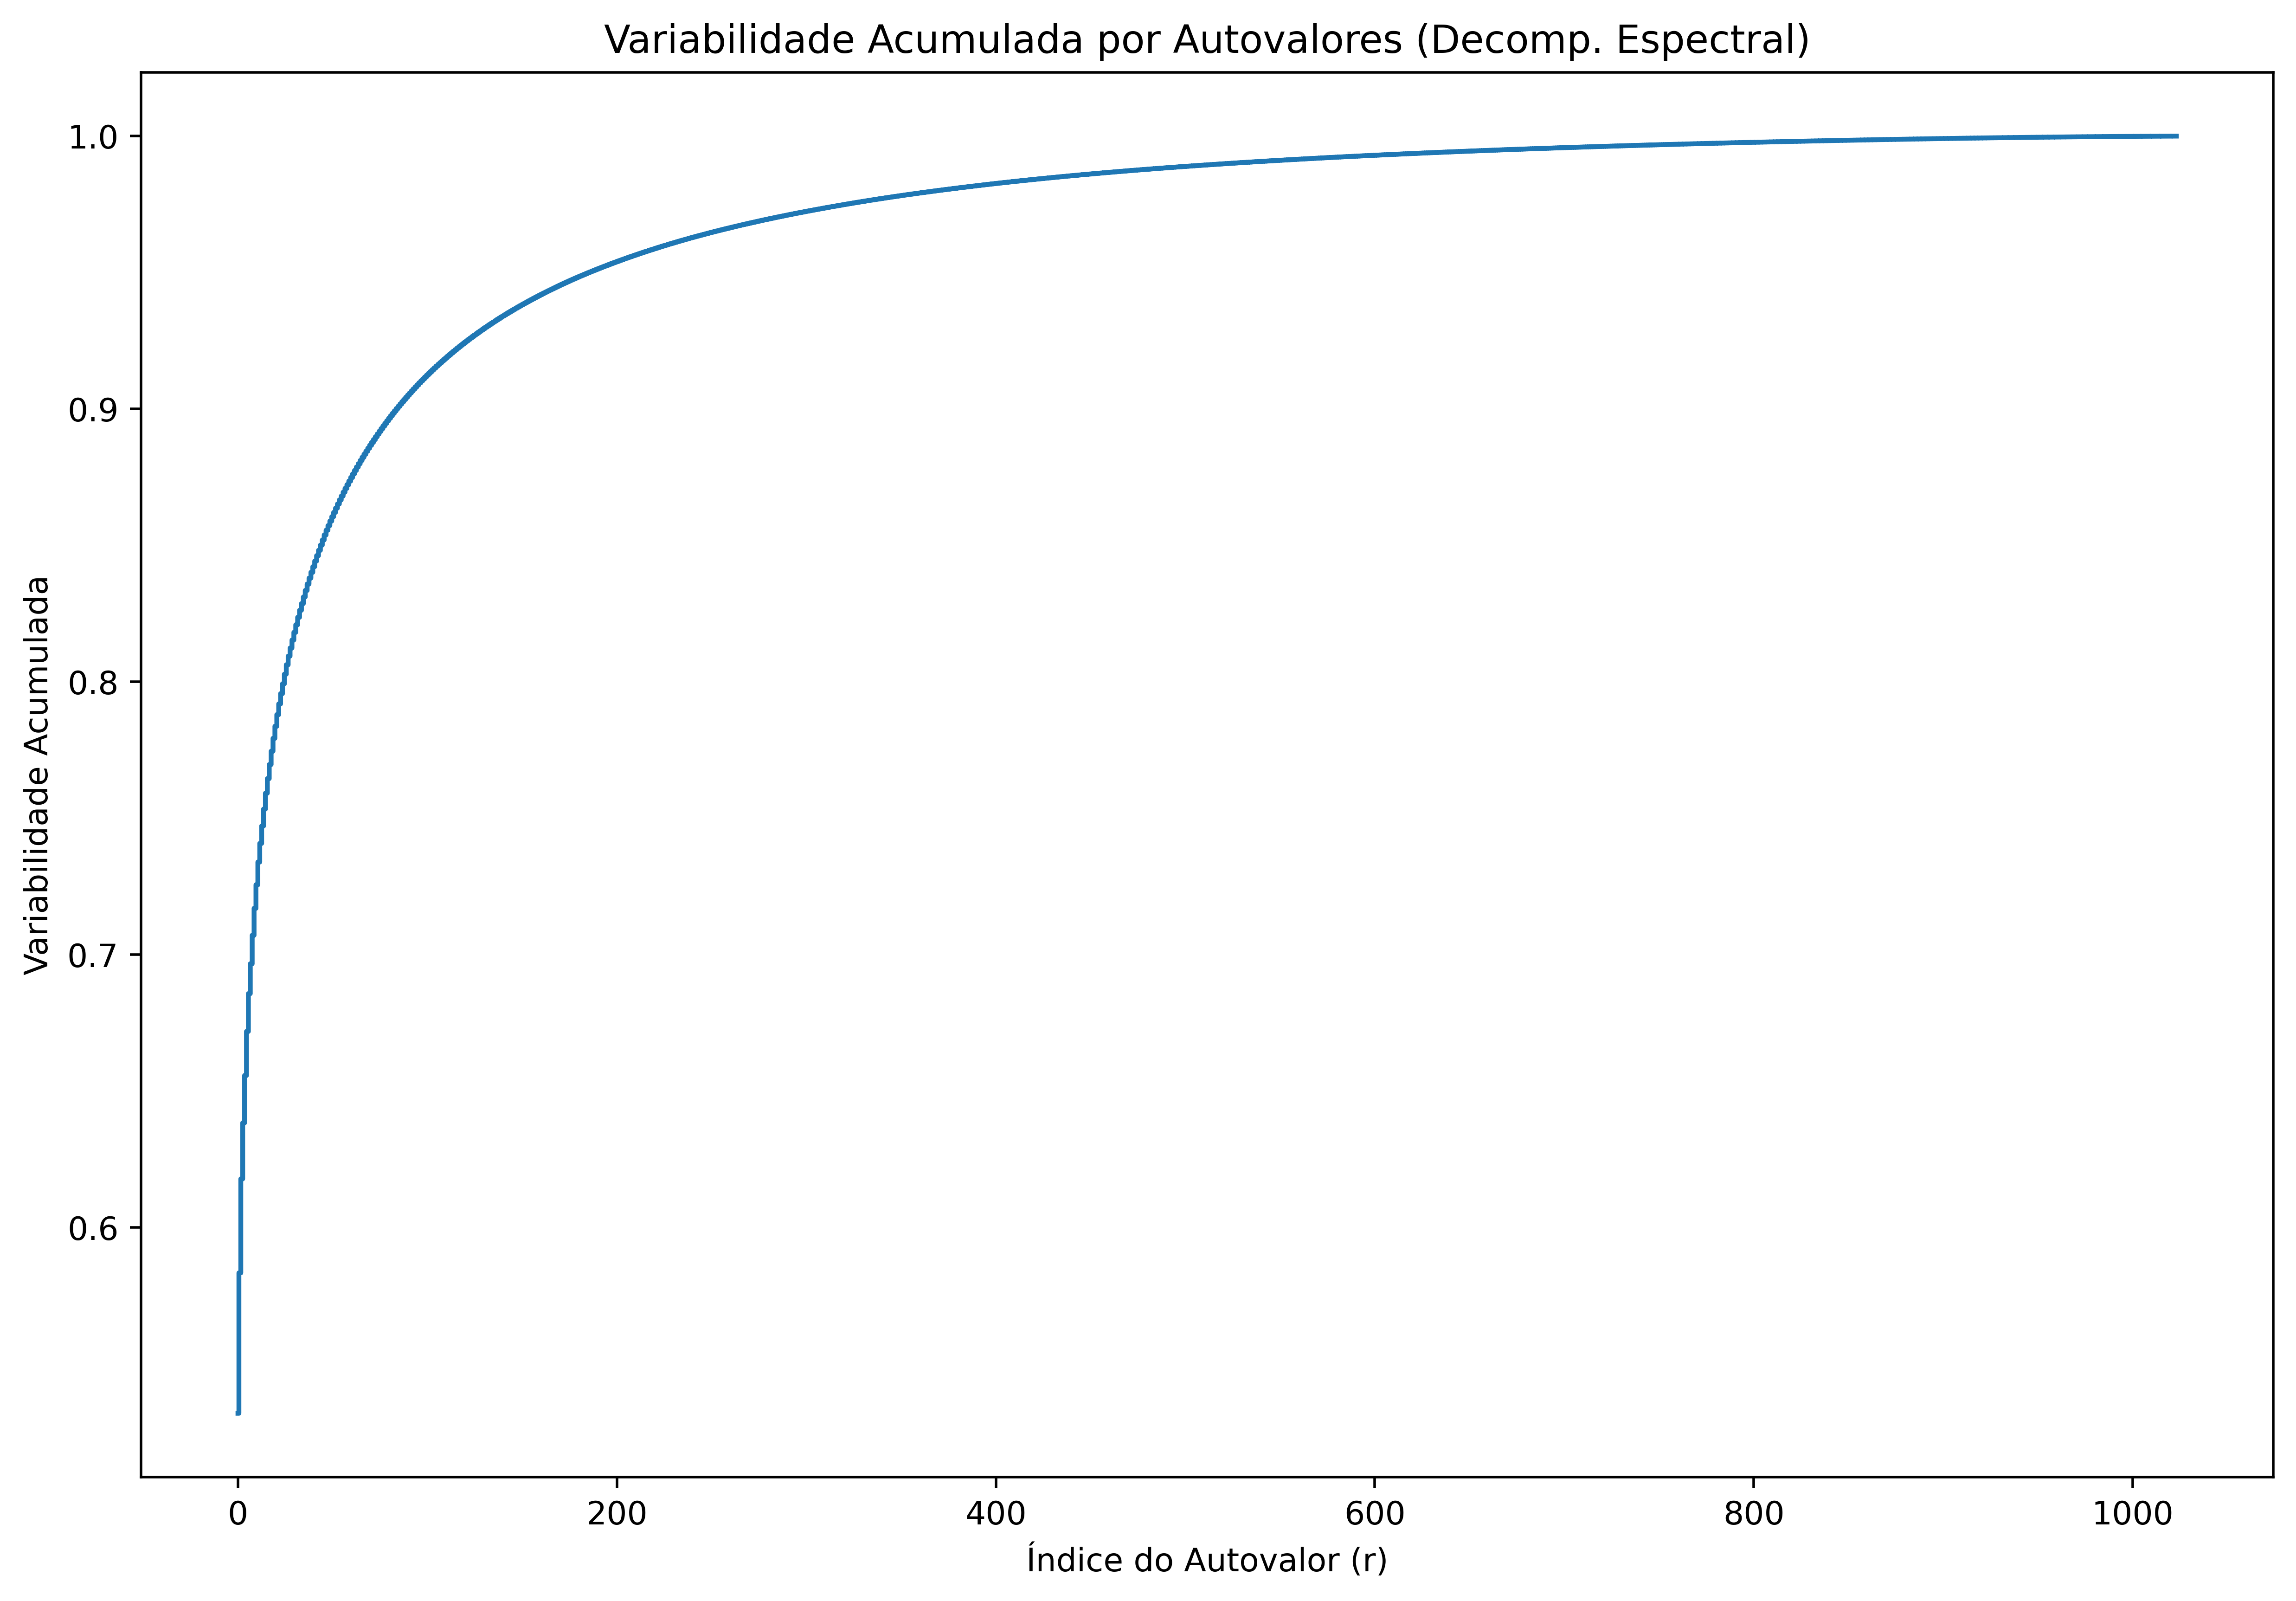
\includegraphics[width=9cm]{var_acu_espectral}
\end{figure}
\end{frame}

\begin{frame}{Experimentos e Resultados}
\begin{figure}[H]
  \centering
  \caption{Gráfico da variabilidade acumulada para 185 autovalores na Decomposição Espectral.}
  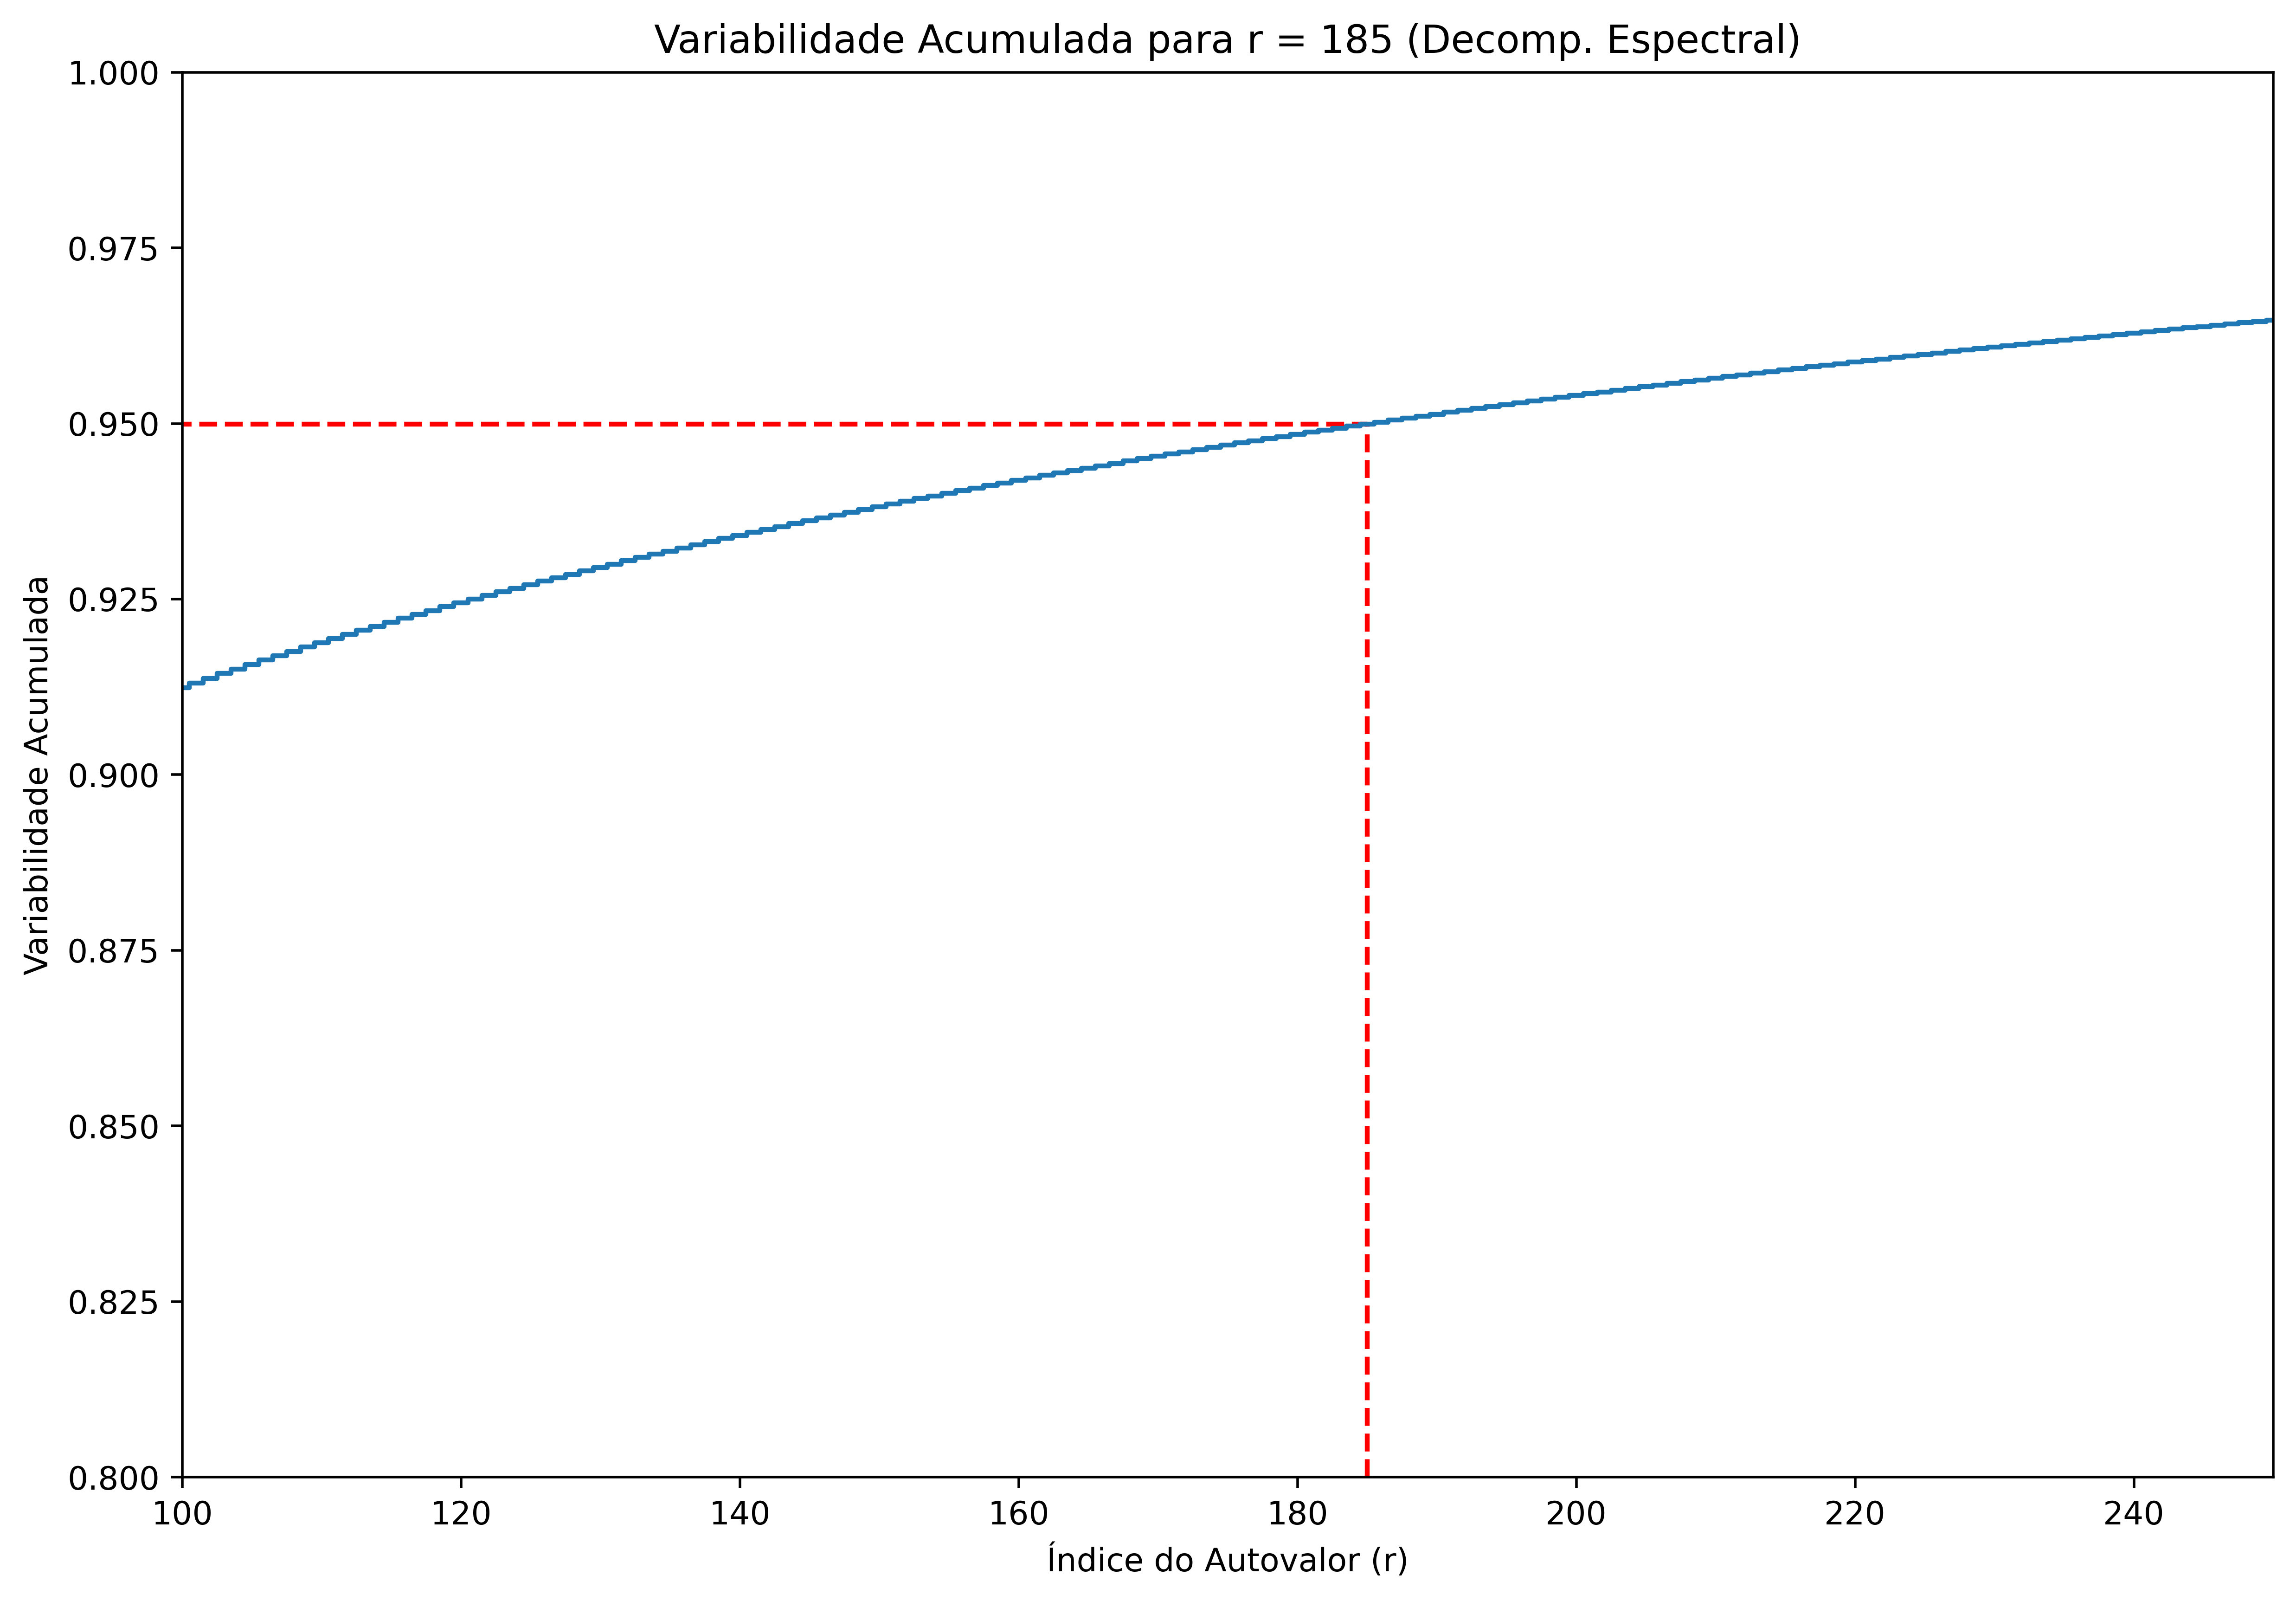
\includegraphics[width=9cm]{var_acu_espectral_185}
\end{figure}
\end{frame}

\begin{frame}{Experimentos e Resultados}
\begin{figure}[H]
  \centering
  \caption{Gráfico da acurácia do algoritmo KNN por valor de r na Decomposição Espectral.}
  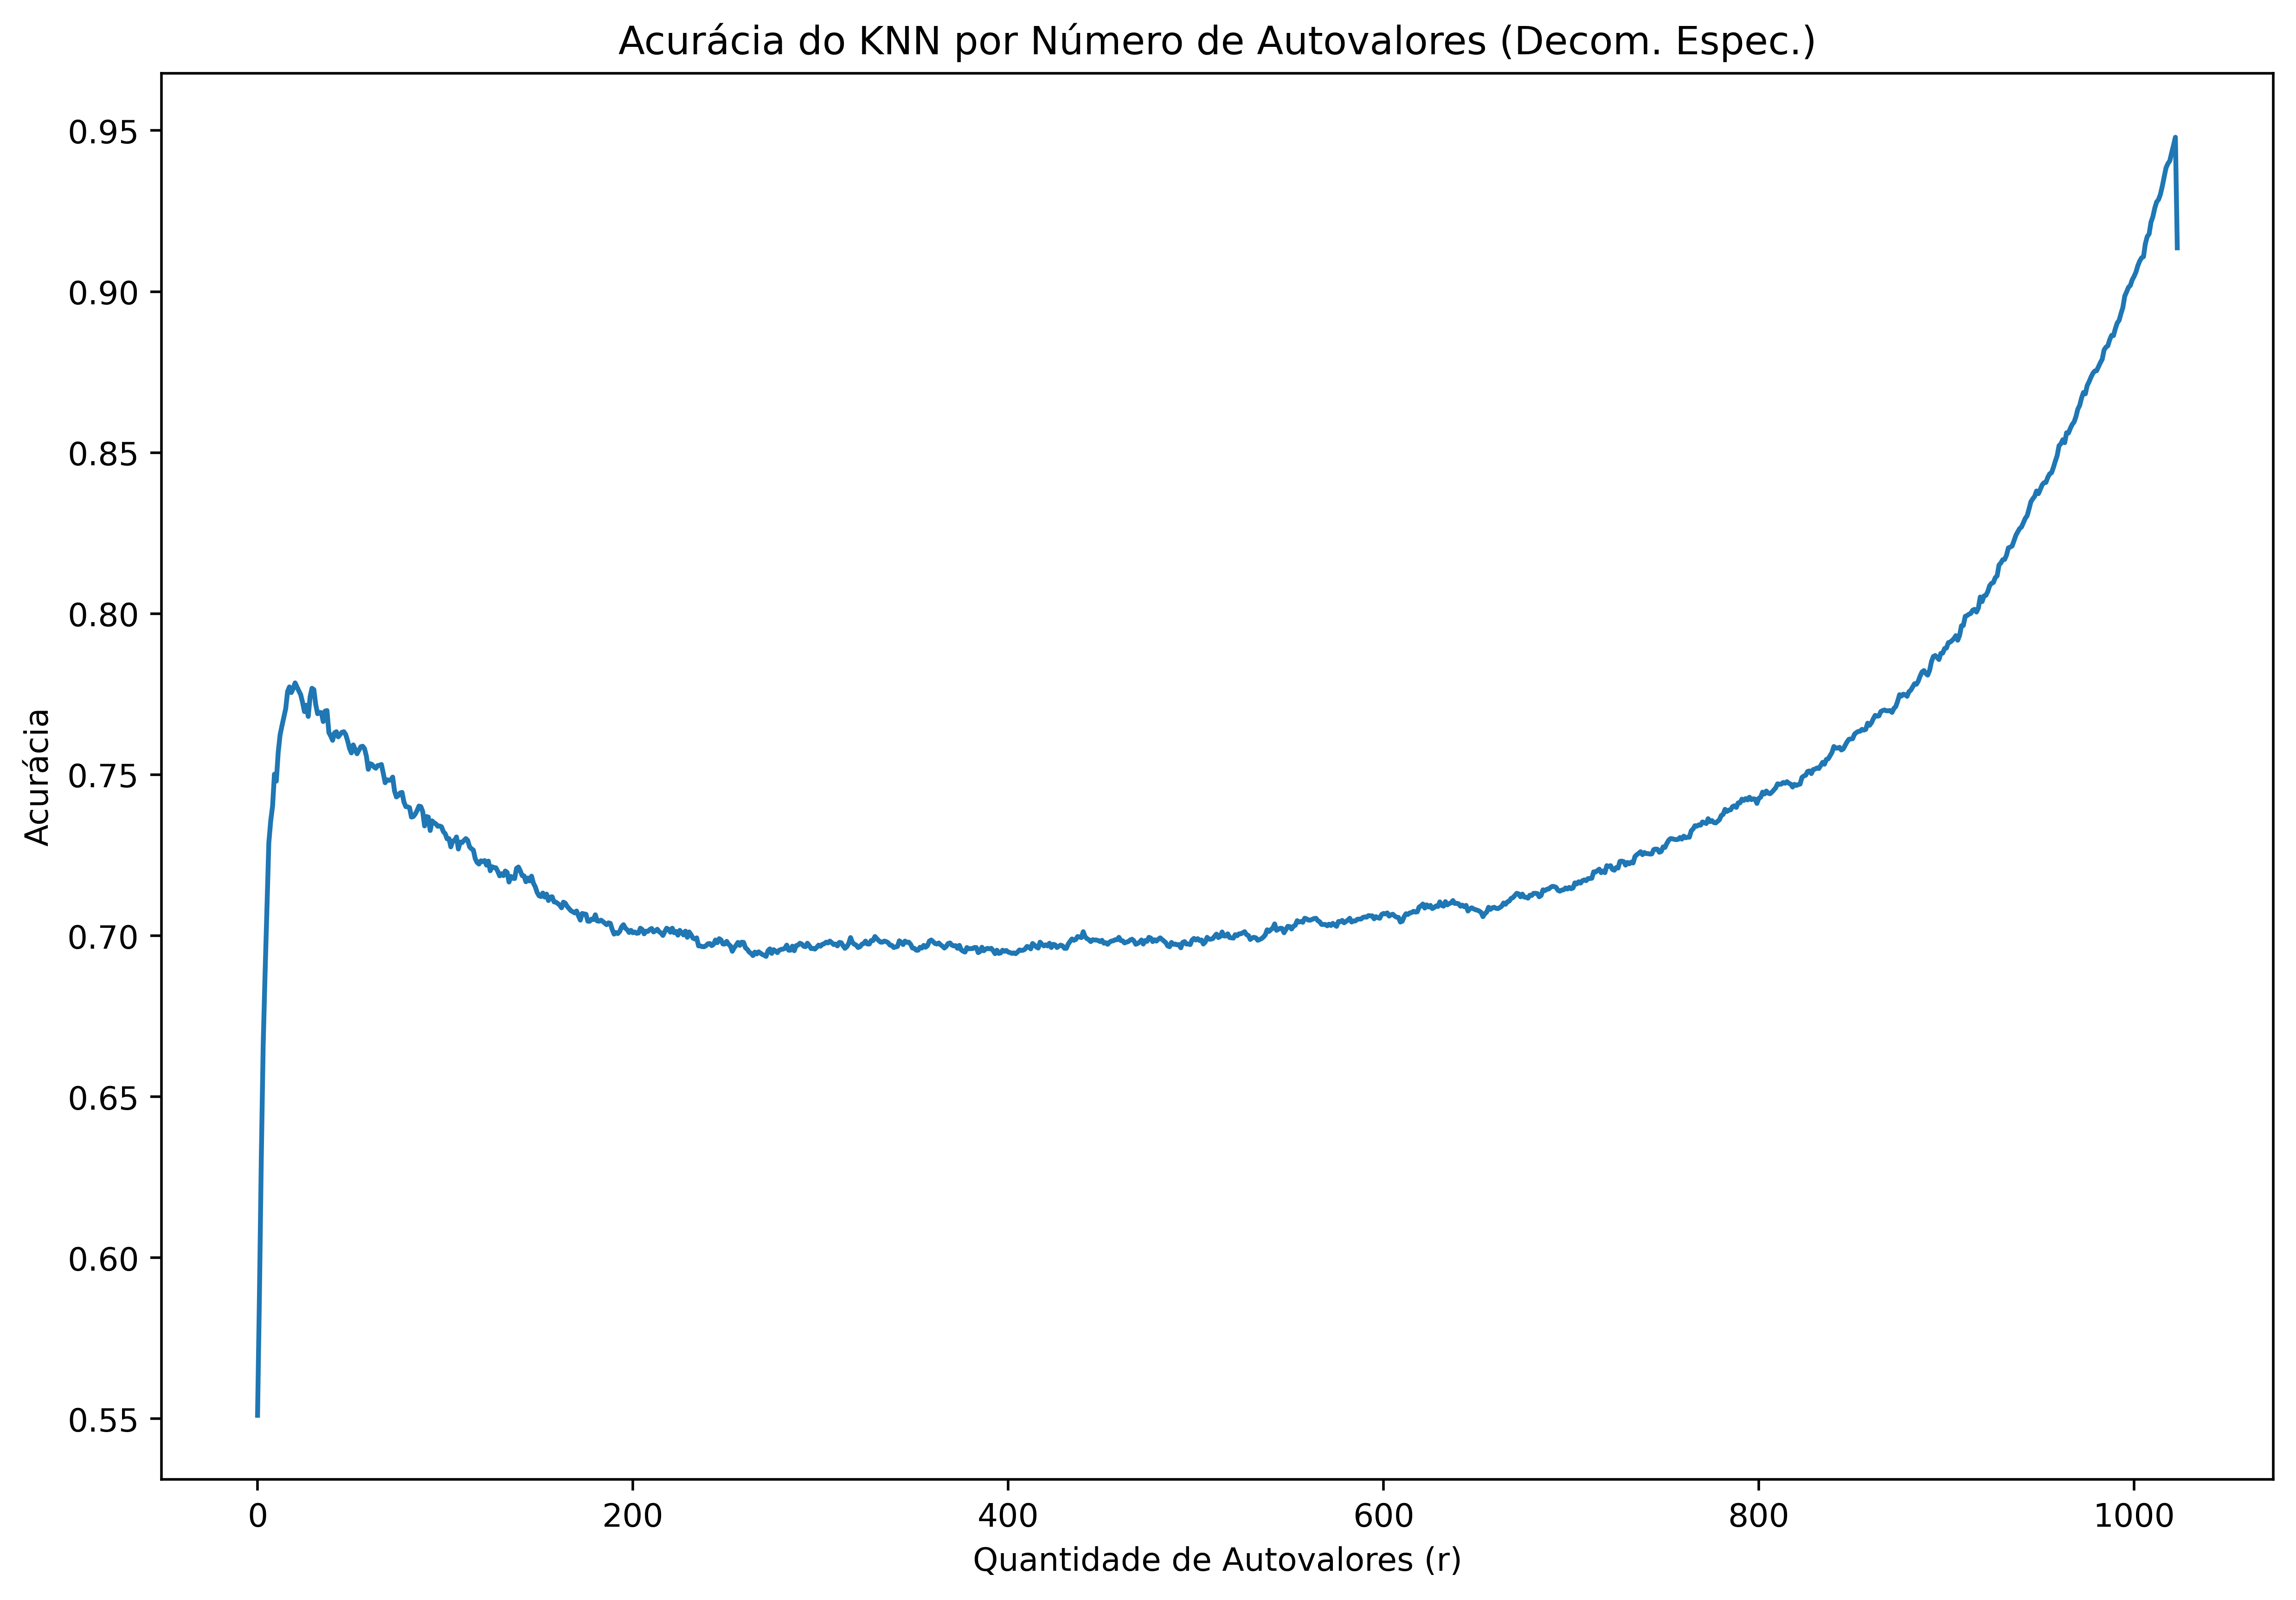
\includegraphics[width=9cm]{acuracia_espectral}
\end{figure}
\end{frame}

\begin{frame}{Experimentos e Resultados}
\begin{figure}[H]
  \centering
  \caption{Gráfico da acurácia do algoritmo KNN na Decomposição Espectral para 20 autovalores.}
  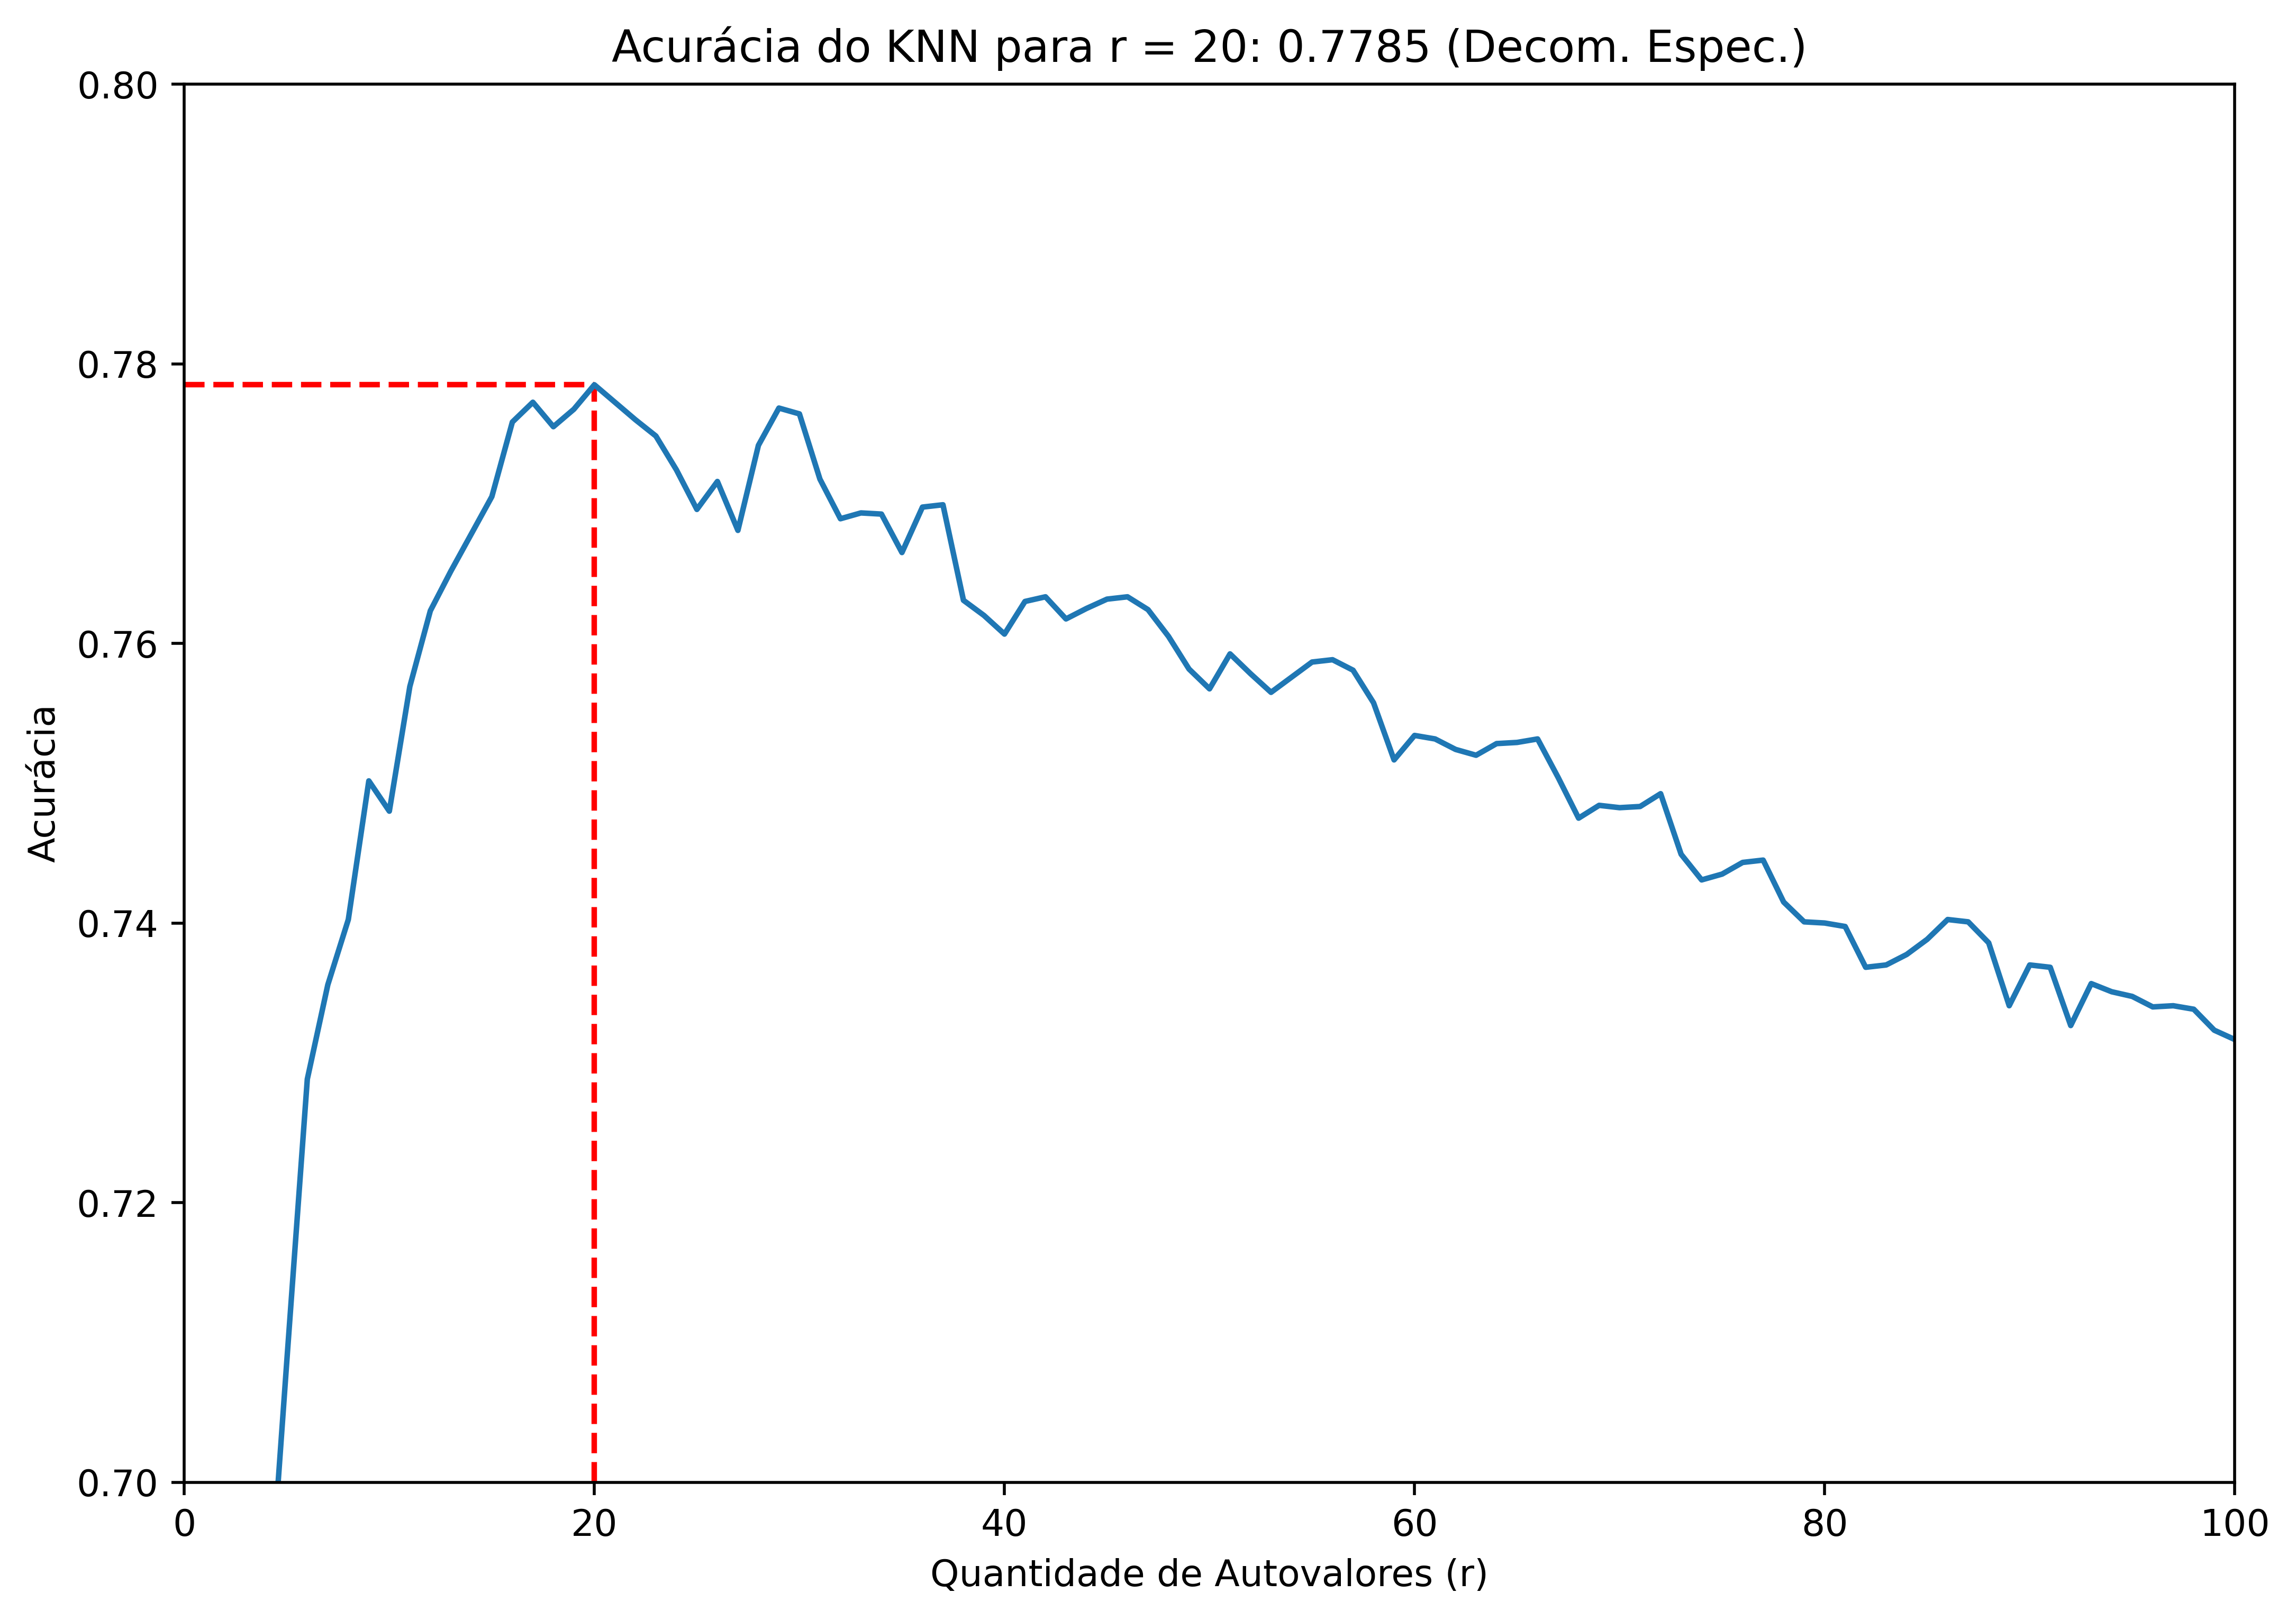
\includegraphics[width=9cm]{acuracia_espectral_20}
\end{figure}
\end{frame}

\begin{frame}{Experimentos e Resultados}
\begin{figure}[H]
  \centering
  \caption{Gráfico da variabilidade acumulada por número de autovalores na SVD.}
  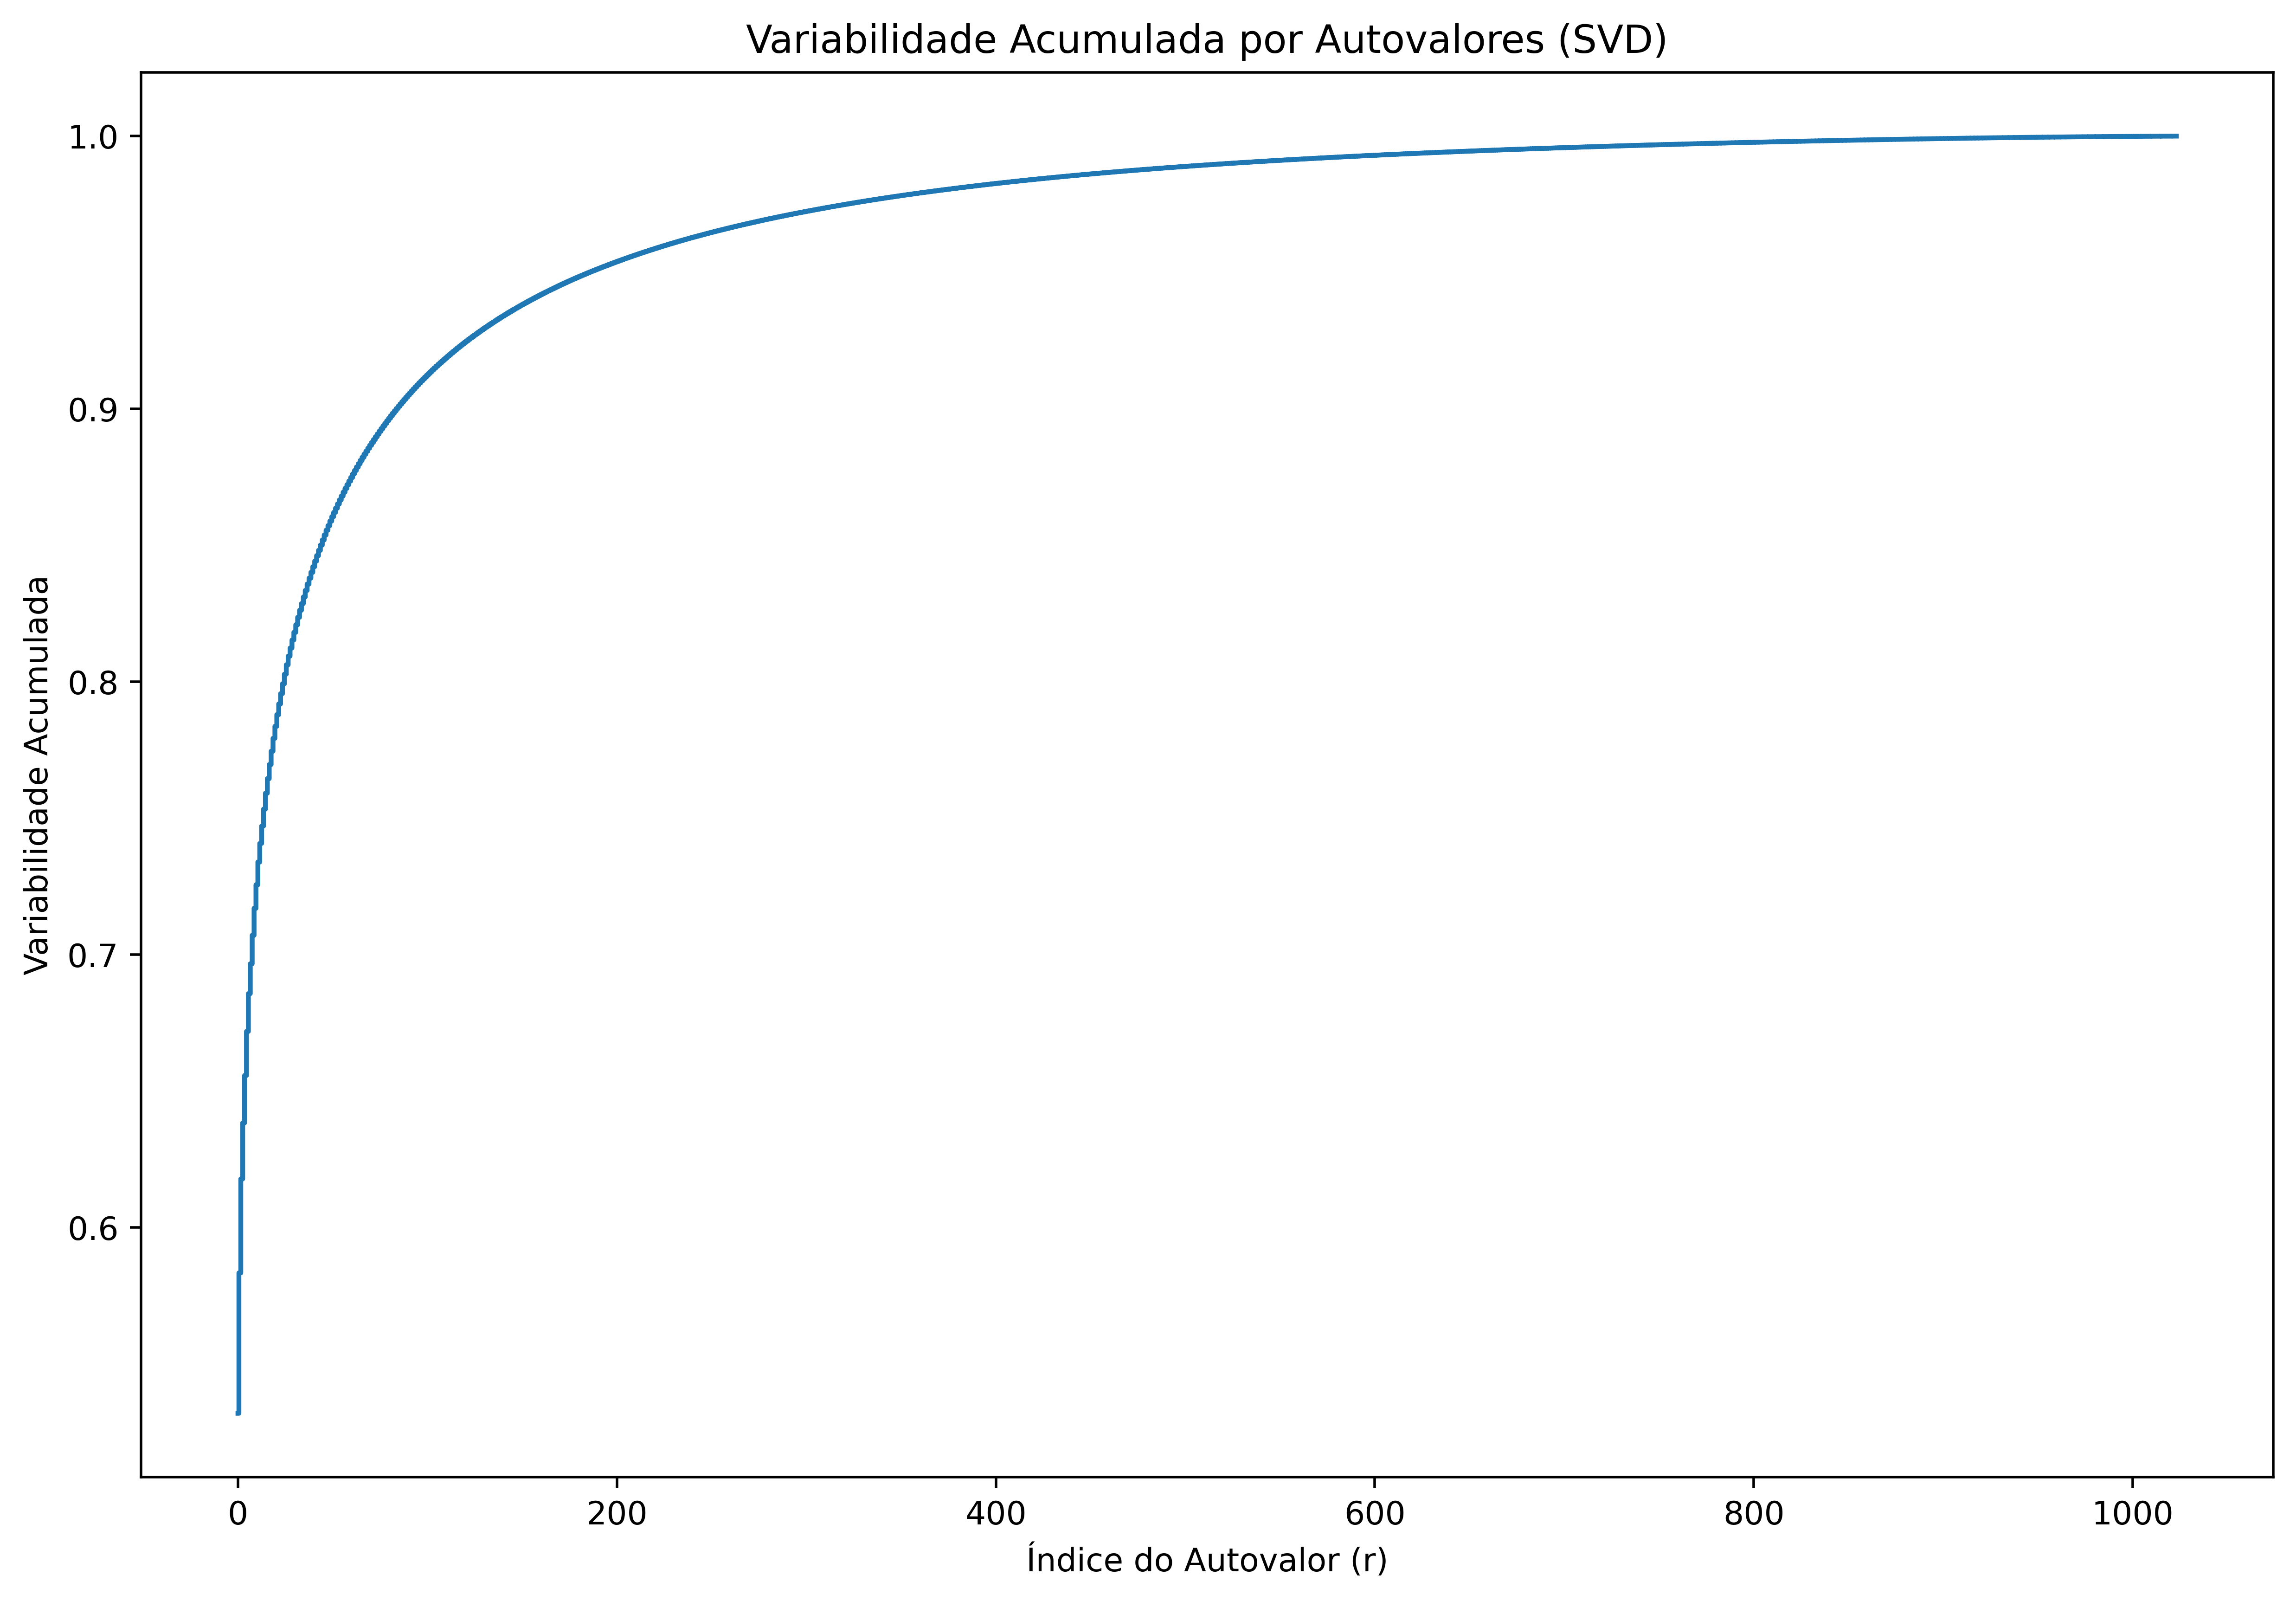
\includegraphics[width=9cm]{var_acu_svd}
\end{figure}
\end{frame}

\begin{frame}{Experimentos e Resultados}
\begin{figure}[H]
  \centering
  \caption{Gráfico da variabilidade acumulada para 185 autovalores na SVD.}
  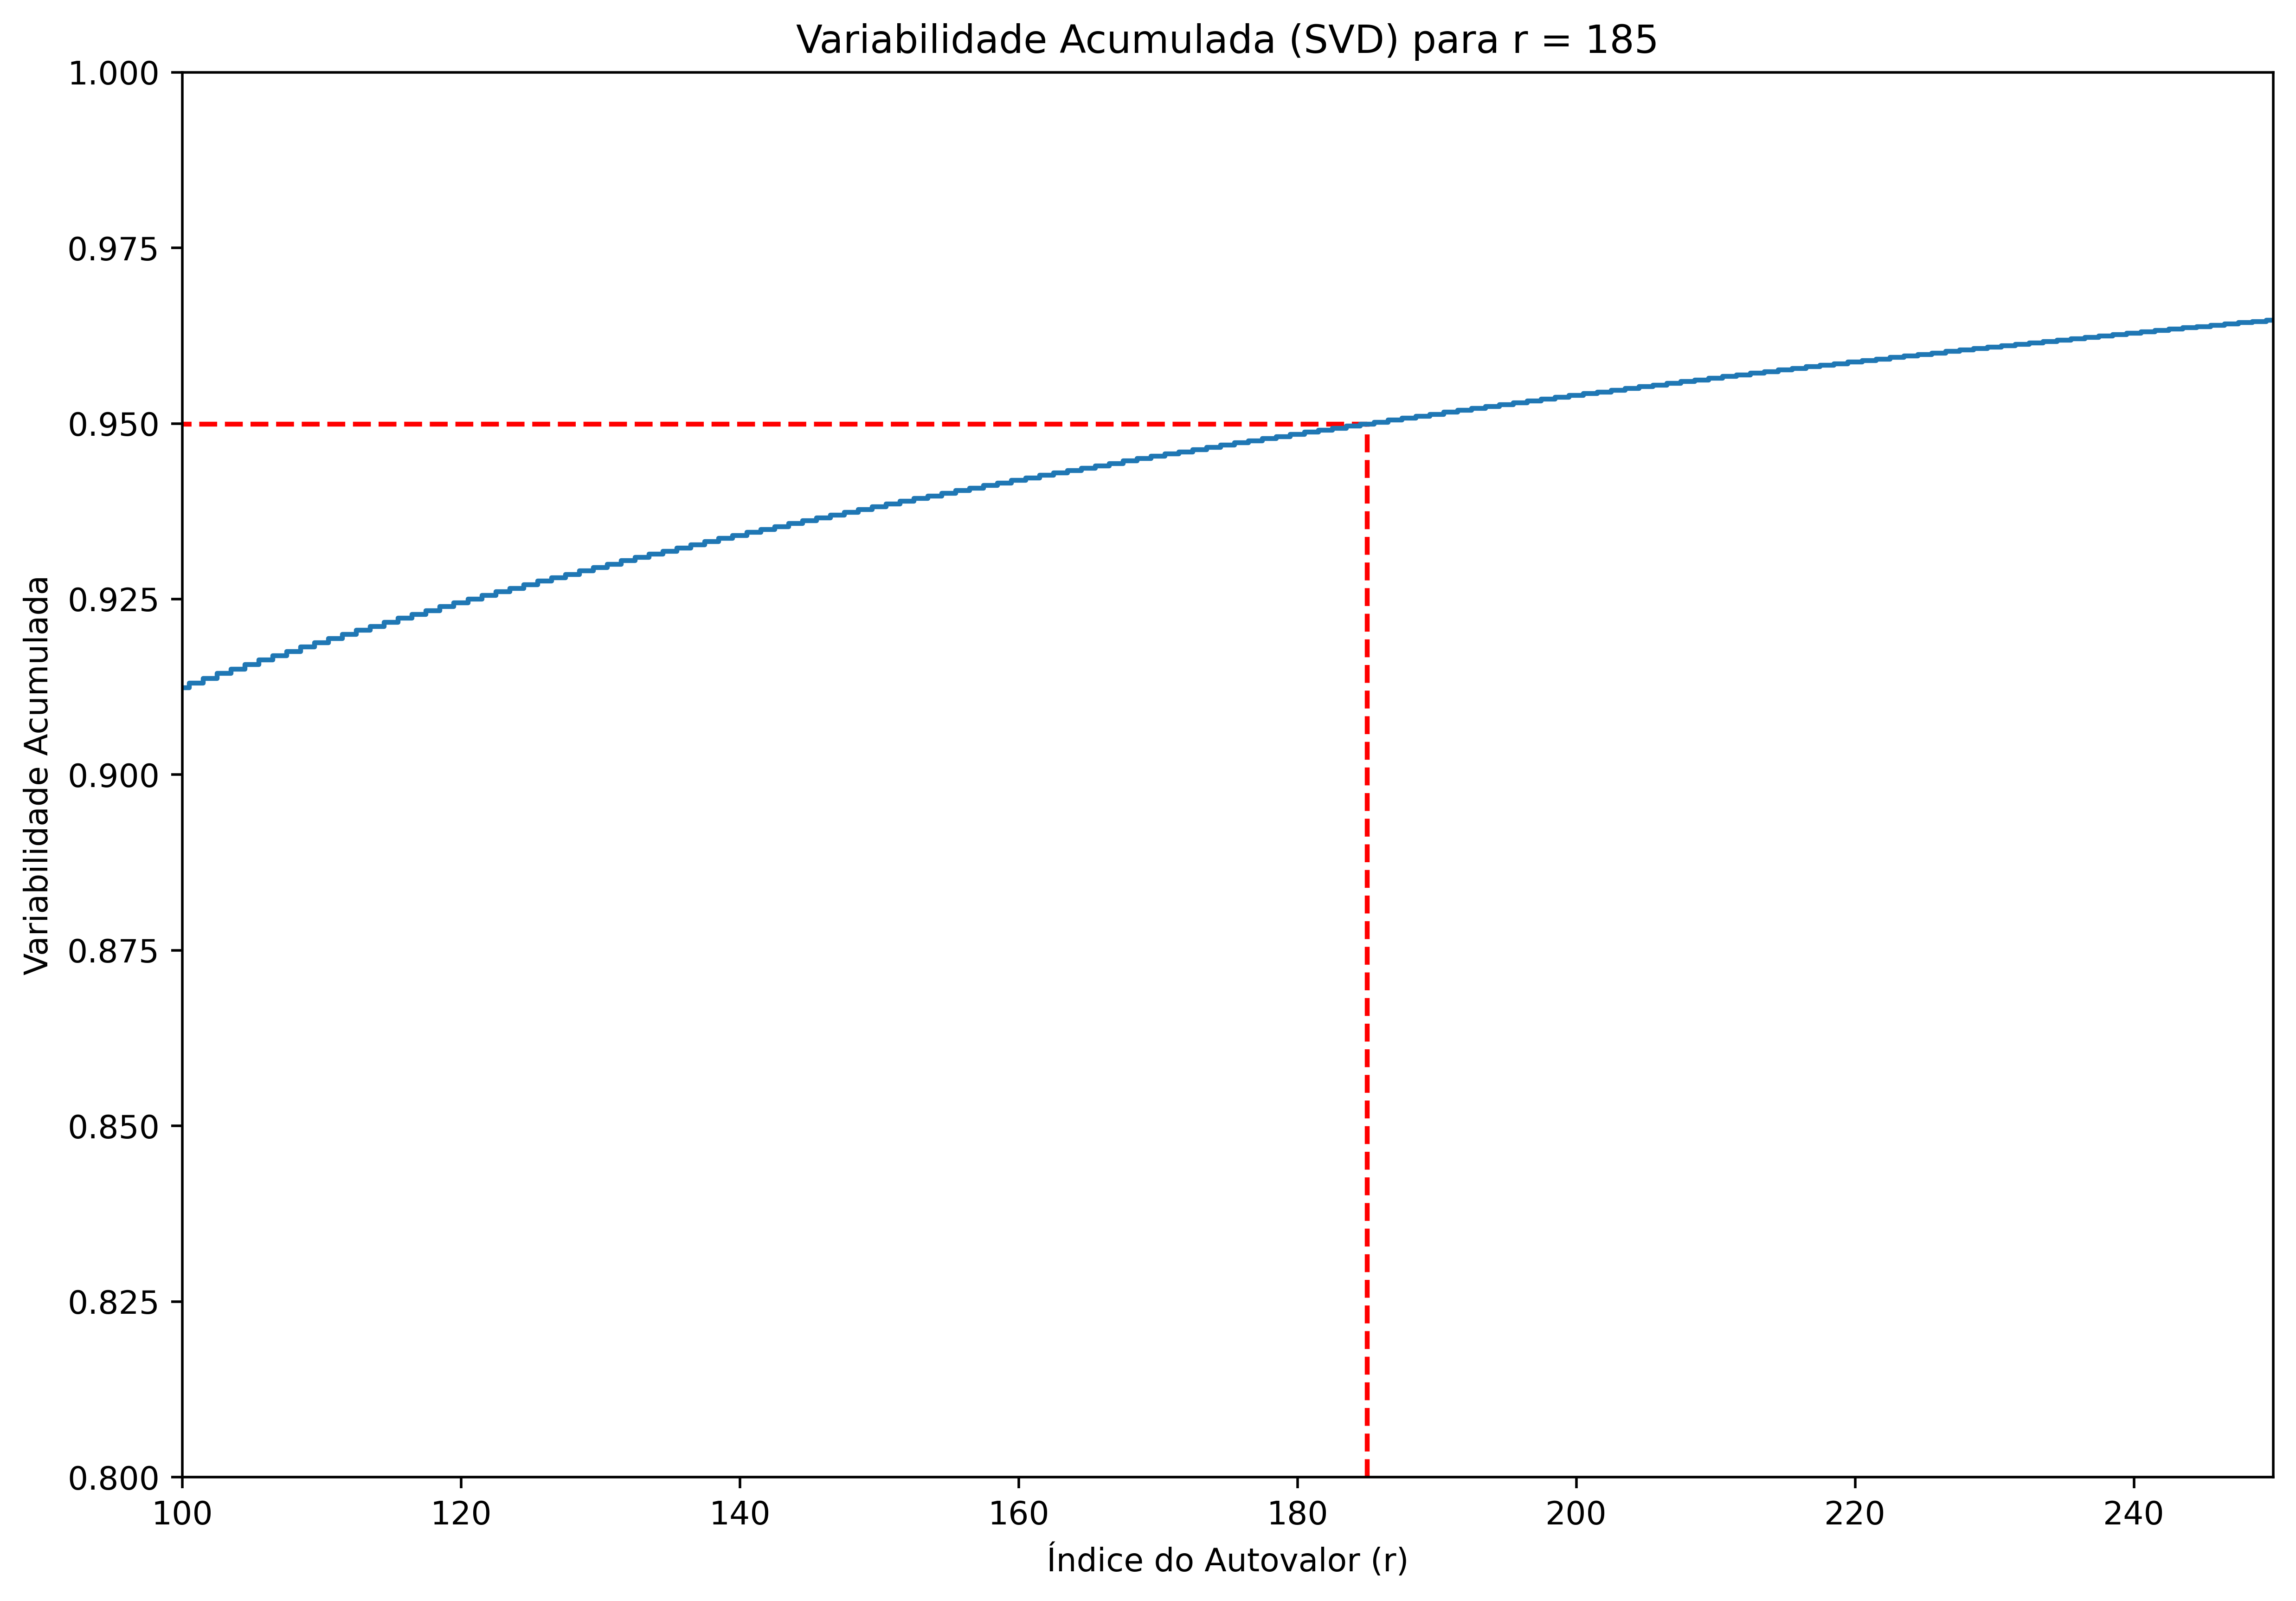
\includegraphics[width=9cm]{var_acu_svd_185}
\end{figure}
\end{frame}

\begin{frame}{Experimentos e Resultados}
\begin{figure}[H]
  \centering
  \caption{Gráfico da acurácia do algoritmo KNN por valor de r na SVD.}
  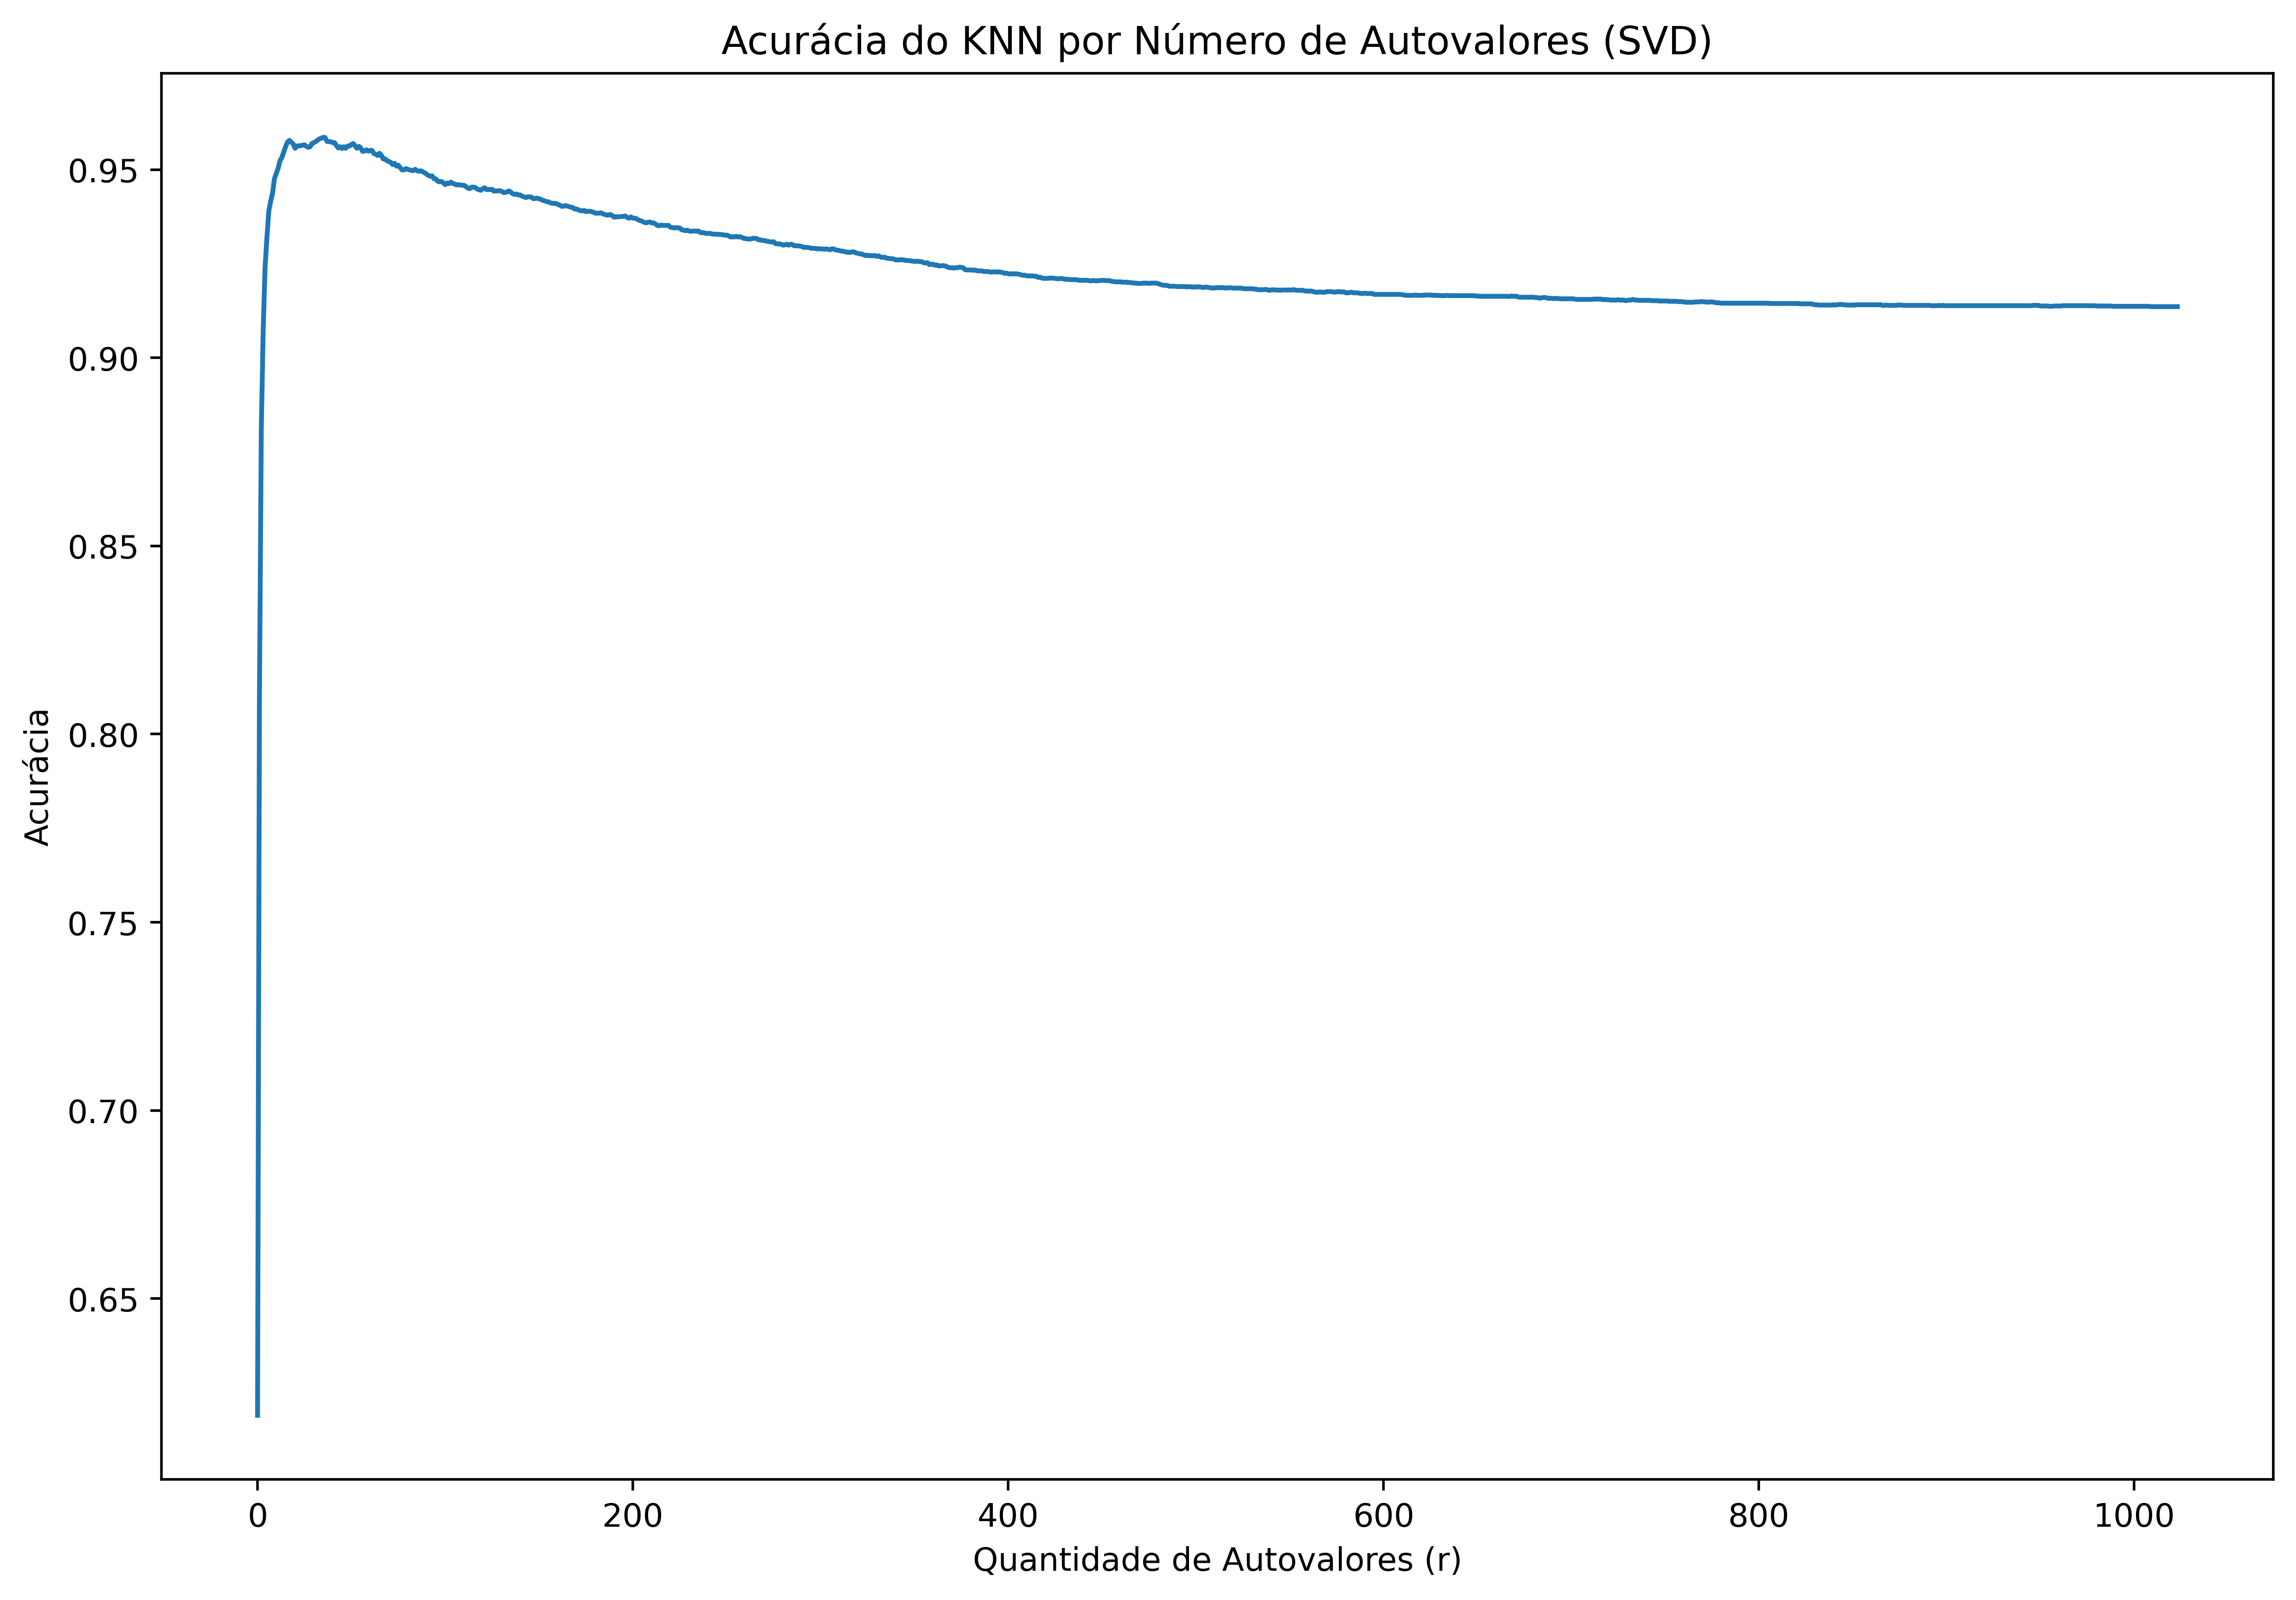
\includegraphics[width=9cm]{acuracia_svd}
\end{figure}
\end{frame}

\begin{frame}{Experimentos e Resultados}
\begin{figure}[H]
  \centering
  \caption{Gráfico da acurácia do algoritmo KNN para 17 autovalores na SVD.}
  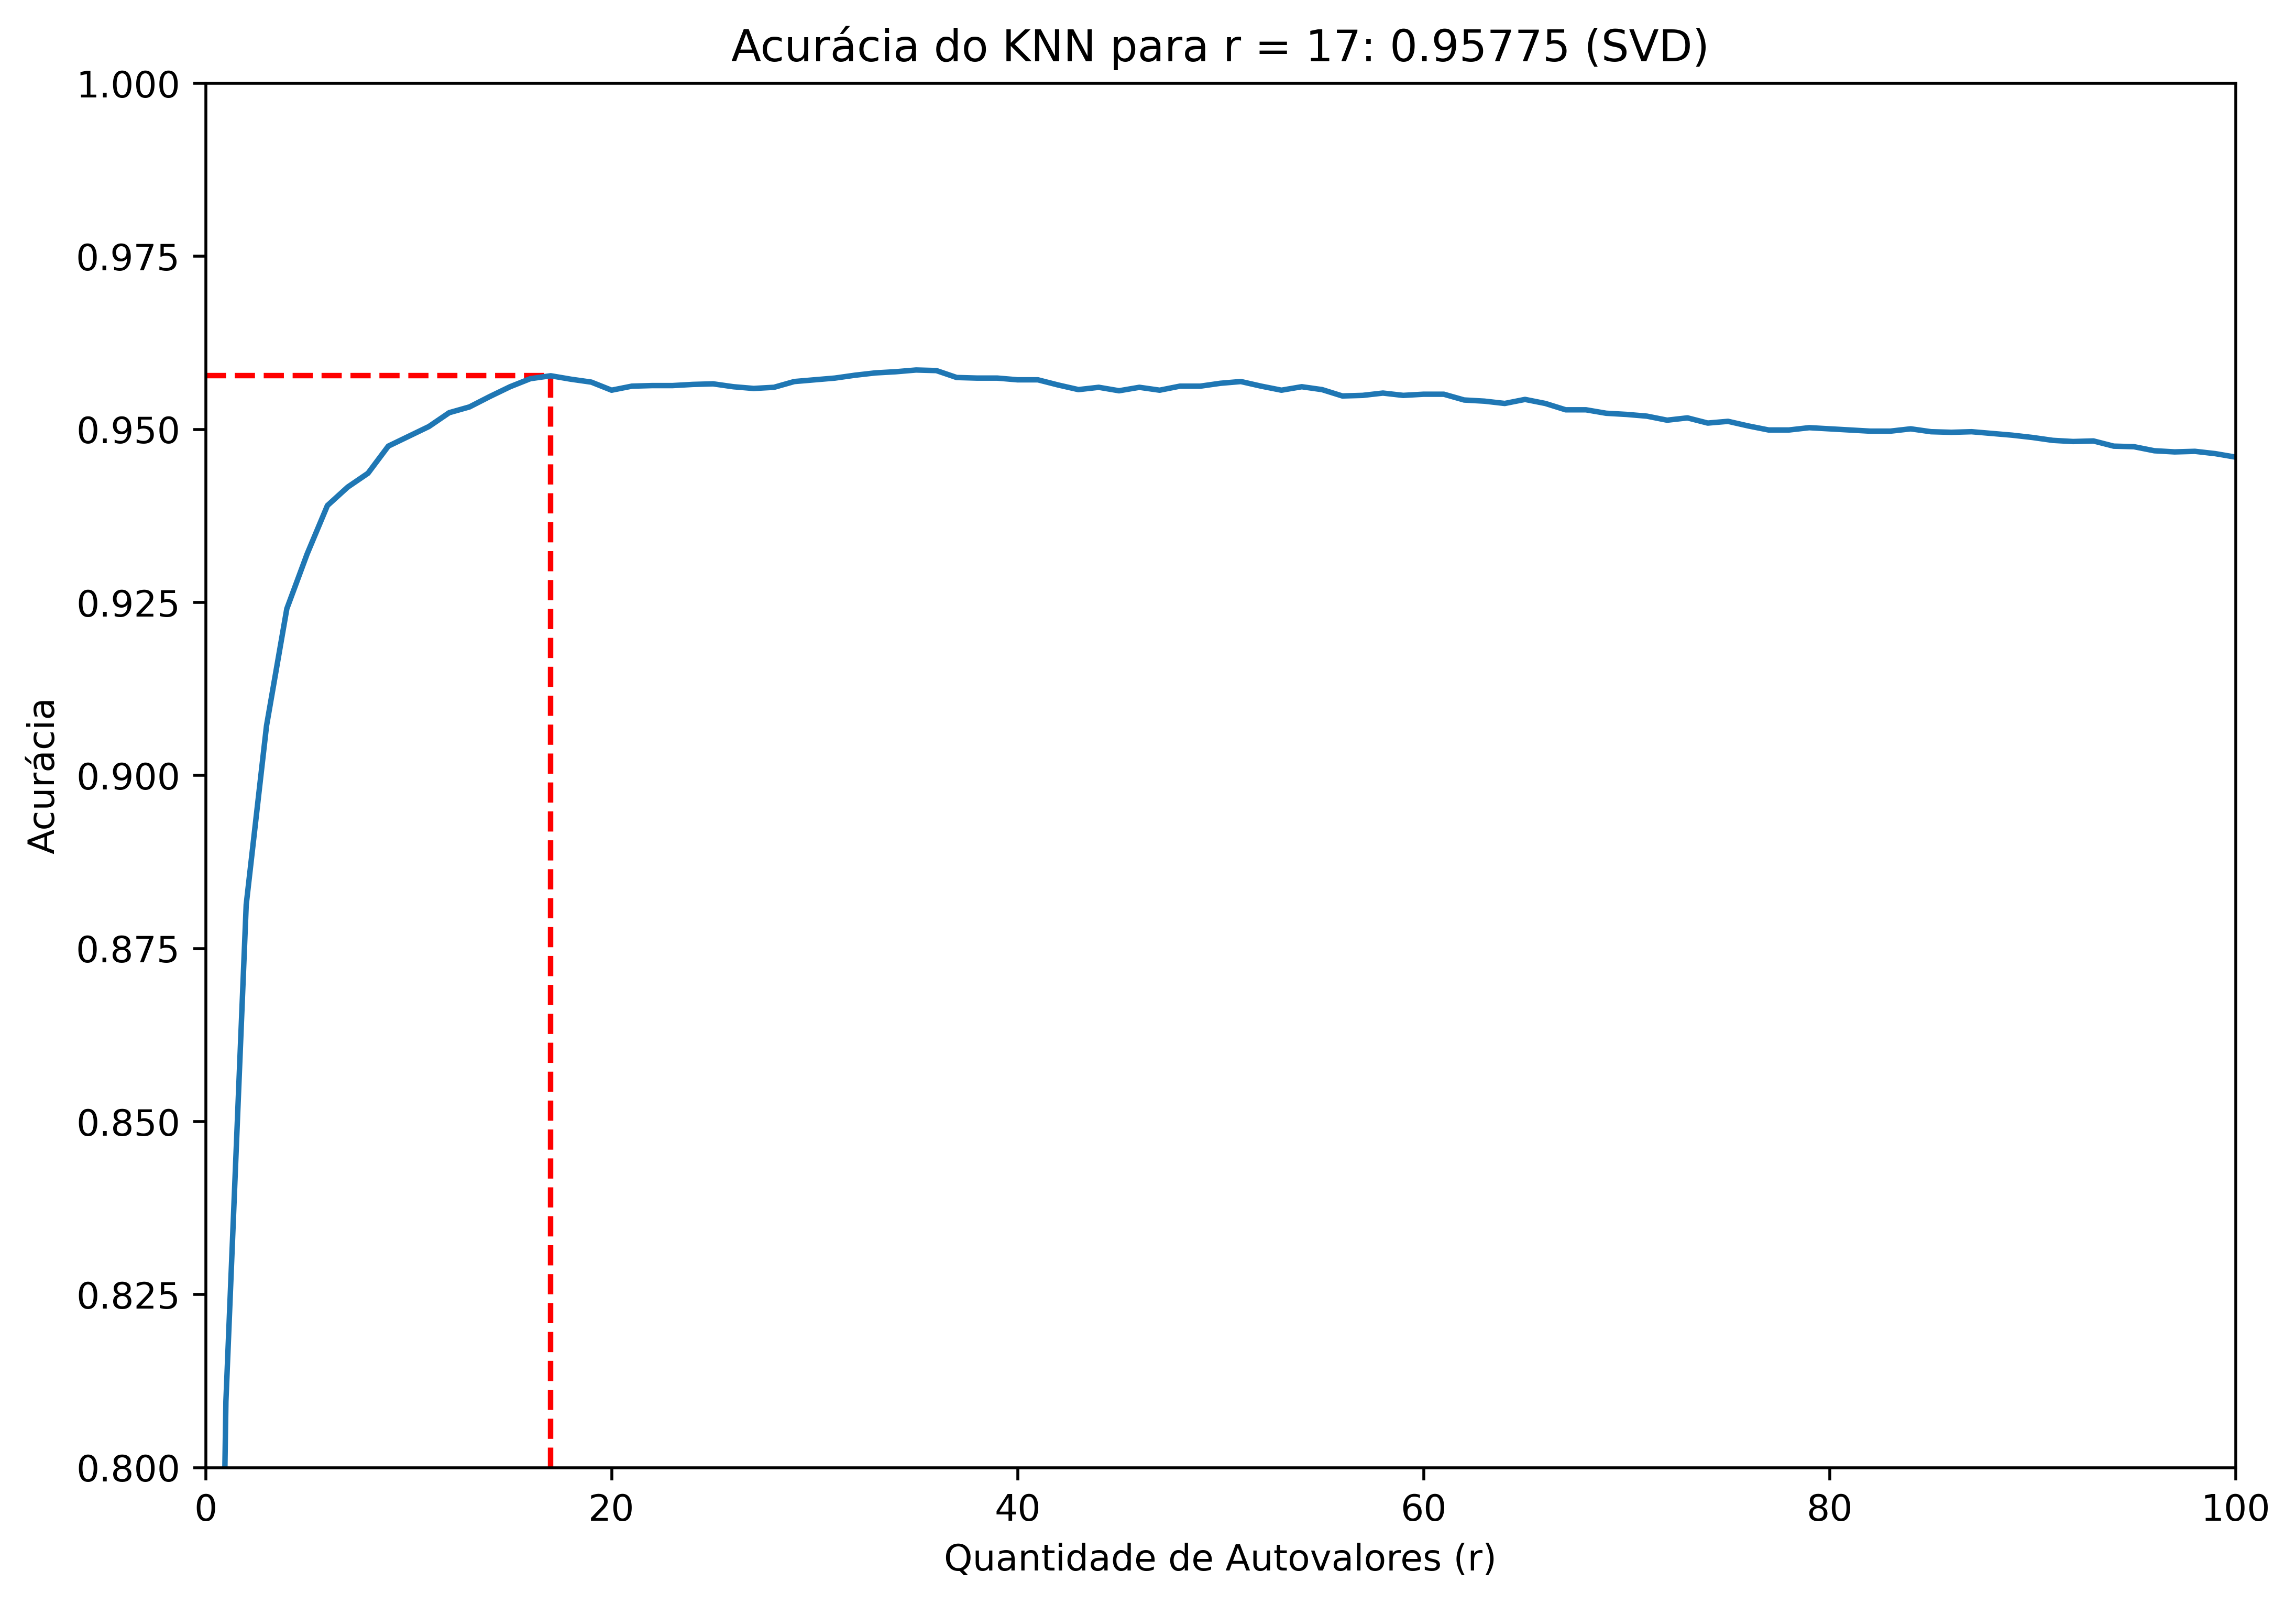
\includegraphics[width=9cm]{acuracia_svd_17}
\end{figure}
\end{frame}

\end{document}
